\section{Data Type}

\subsection{\texttt{MasterBoard}}

\subsubsection{Description}
\texttt{MasterBoard} represents a single whiteboard on the server. The instance is held by several \texttt{User} objects editing the board, which are mutually stored in the \texttt{MasterBoard} object; in other words, the board is aware of its editors and the editors are aware of the board.

\subsubsection{Fields}
\begin{itemize}
\item \texttt{final String name} - The name of the board in the grammar format \texttt{NAME}.
\item \texttt{final int id\_num} - The unique identification number of the board.
\item \texttt{static final AtomicInteger nextID} - The identification number of the successive board to be created.
\item \texttt{final static int Y\_SIZE, X\_SIZE} - The X and Y dimensions of the whiteboard.
\item \texttt{final ArrayList<WhiteLine> strokes} - A list of the strokes drawn on the whiteboard. The ordering of these strokes corresponds to the sequence in which modifications were made on the server and the layering of the segments.
\item \texttt{final ArrayList<User> users} - A list of editors currently modifying the board.
\end{itemize}

\subsubsection{Methods}
\begin{itemize}
\item \texttt{WhiteLine[] allStrokes()} - Returns all the strokes that have been made on the board thus far by locking on \texttt{strokes} list.
\item \texttt{void makeStroke(Stroke stroke)} - Adds the new \texttt{stroke} while locking on the \texttt{strokes} list. Proceeds to call \texttt{incorporateStroke()} on each user while locking on the \texttt{users} list.
\item \texttt{void addUser(User user)} - Adds the new \texttt{user} while locking on the \texttt{users} list.
\item \texttt{void removeUser(User user)} - Removes the user \texttt{user} while locking on the \texttt{users} list.
\item \texttt{User[] getUsers()} - Returns all current editors while locking on the \texttt{users} list.
\item \texttt{String getName()} - Returns the name of the whiteboard.
\item \texttt{int getID()} - Returns the unique identification number of the board.
\item \texttt{String toString()} - Returns the properties of the board in the form of a \texttt{BOARD\_INFO} message.
\item \texttt{boolean equals(Object other)} - Compares boards for equality on the basis of ID number.
\item \texttt{int hashCode()} - Returns the identification number of board added to 1000.
\end{itemize}

\subsubsection{In Action}
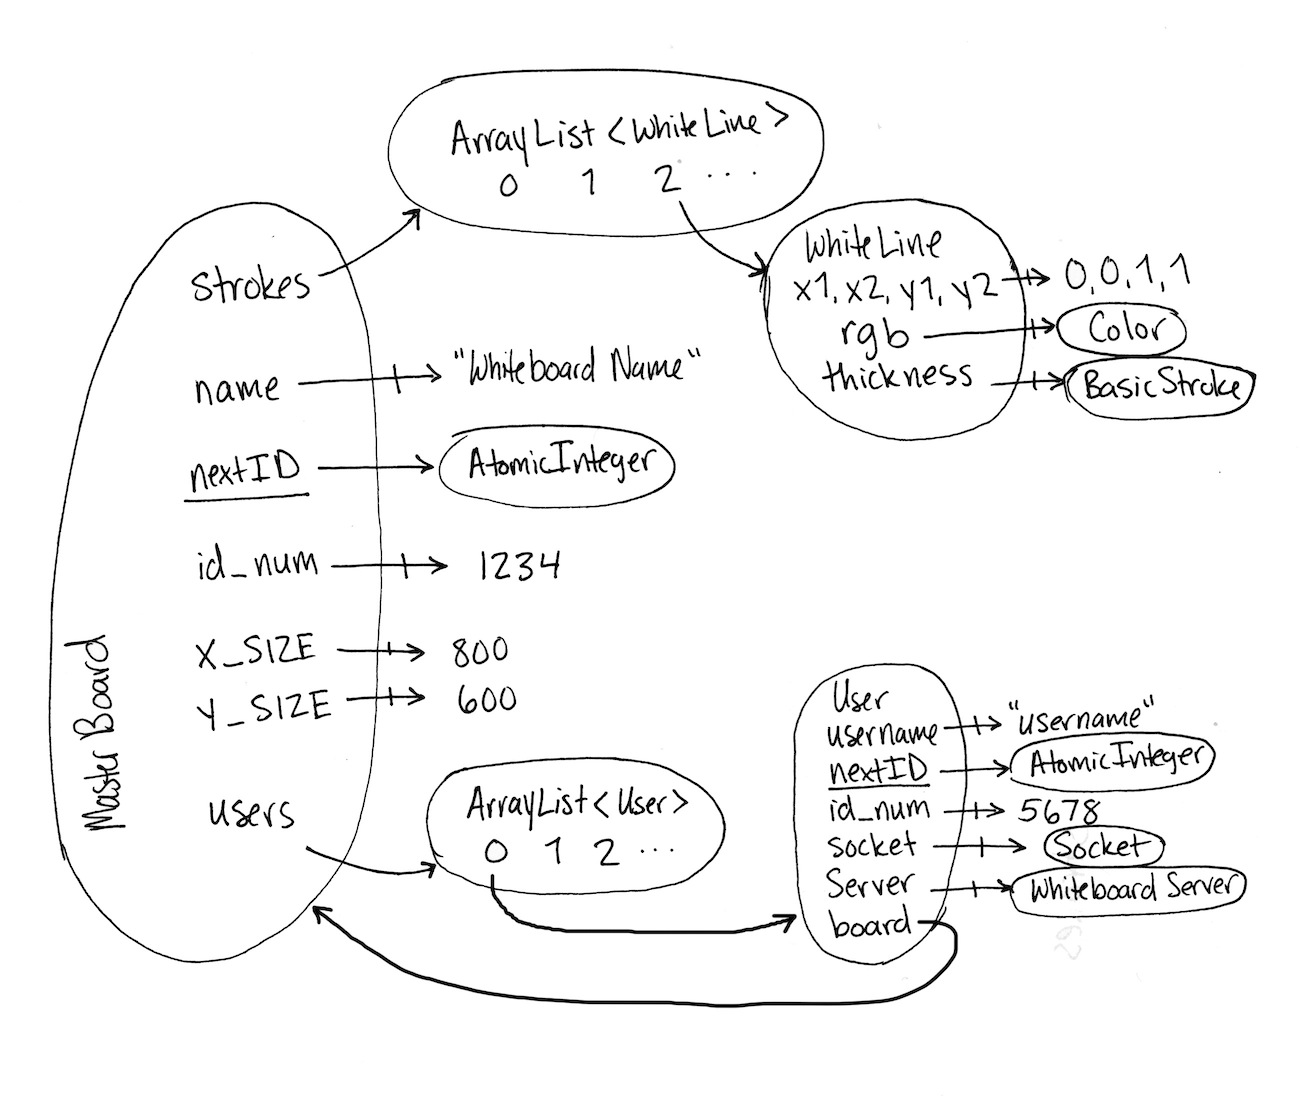
\includegraphics[keepaspectratio=1,width=6in]{img/wb-snapshot.jpg}


\subsection{\texttt{User}}

\subsubsection{Description}
Each instance of \texttt{User} represents a separate client connected to the server. \texttt{User} is not only responsible for storing properties that pertain to the client; it also facilitates the socket communication and request handling for each client.

\subsubsection{Fields}
\begin{itemize}
\item \texttt{final Whiteboard Server} - The main server instance is stored for later global calls.
\item \texttt{MasterBoard board} - The current board being edited by the user. A null value indicates that no board is selected.
\item \texttt{final String username} - The unique acquired username assigned by the server after a username request has been made.
\item \texttt{final int id\_num} - The unique identification number of the user.
\item \texttt{static final AtomicInteger nextID} - The identification number of the successive user to be created.
\item \texttt{final Socket socket} - The socket corresponding to the client application represented by the \texttt{User} instance. The input and output streams are contained within.
\item \texttt{BlockingQueue queue} - The queue containing all outgoing messages to the connected client.
\end{itemize}

\subsubsection{Methods}
\begin{itemize}
\item \texttt{void incorporateBoard(MasterBoard board)} - Queues a \texttt{BRD\_INFO} message to be sent to the client with priority. This method is called by the main \texttt{WhiteboardServer} on all \texttt{User} instances once the request for a new board has been processed.
\texttt{void forgetBoard(MasterBoard board)} - Queues a \texttt{BRD\_DEL} message to be sent to the client with priority. This method is called by the main \texttt{WhiteboardServer} on all \texttt{User} instances once the request to remove a whiteboard has been processed.
\item \texttt{void incorporateStroke(WhiteLine stroke)} - Queues a \texttt{STROKE} message to inform the client of a new stroke drawn on the current board.
\item \texttt{void handleRequest()} - Runs in a background thread and takes care of all incoming requests from the client. Appropriate actions are taken for each request, either with the \texttt{server} or on the \texttt{board}.
\item \texttt{void selectBoard(int boardID)} - This method is called upon receiving a \texttt{SEL} command from the client. The user removes itself from the current board by calling \texttt{removeUser(this)} on the locked \texttt{board}, replacing \texttt{board} with on acquired from \texttt{server.getBoard(boardID)} and calling \texttt{addUser(this)} on the new reference. All queued \texttt{STROKE} are removed since they pertain to the old board. The method finally calls \texttt{board.allStrokes()} to queue all previously drawn strokes for the new board to be sent to the client.
\item \texttt{String getName()} - Returns the username of the connected client.
\item \texttt{int getID()} - Returns the unique identification number of the connected client.
\item \texttt{int compareTo(Object other)} - Compares users for ordering on the basis of usernames.
\item \texttt{int equals(Object other)} - Compares users for equality on the basis of identification numbers.
\item \texttt{int hashCode()} - Returns the identification number of the user added to 2000.
\item \texttt{String toString()} - Returns the uername and ID number of the user in string format.
\end{itemize}


\subsection{\texttt{WhiteLine}}

\subsubsection{Description}
\texttt{WhiteLine} is a simple class designed to represent a drawn stroke on a whiteboard. It is used by the \texttt{MasterBoard} class on the server side and the \texttt{ClientView} class on the client side. Due to the frequent need to work with lines and the neatness of working with a single object containing the multiple properties of the line -- location, color, thickness -- we decided to have a dedicated class. The class is immutable, as all its properties are themselves immutable and stored upon construction.

\subsubsection{Fields}
\begin{itemize}
\item \texttt{final int x1, y1, x2, y2} - The coordinates of the line, which spans from \texttt{(x1,y1)} to \texttt{(x2,y2)}.
\item \texttt{final java.awt.Color color} - The color of the line. The \texttt{Color} object allows greater versatility over storing individual RGB values, as Java provides multiple methods for specifying colors. This is especially useful for using a \texttt{JColorChooser}.
\item \texttt{final java.awt.BasicStroke thickness} - The thickness of the line will be specified as a number within the range [1,10]. Numbers from this qualitative scale will be mapped to floating-point thicknesses and a \texttt{BasicStroke} object will be constructed internally.
\end{itemize}

\subsubsection{Methods}
\begin{itemize}
\item \texttt{int getX1()} - Returns the X-coordinate of the origin of the line.
\item \texttt{int getY1()} - Returns the Y-coordinate of the origin of the line.
\item \texttt{int getX2()} - Returns the X-coordinate of the terminus of the line.
\item \texttt{int getY2()} - Returns the Y-coordinate of the terminus of the line.
\item \texttt{java.awt.Color getColor()} - Returns the \texttt{Color} object corresponding to the line.
\item \texttt{java.awt.BasicStroke getThickness()} - Returns the \texttt{BasicStroke} object corresponding to the thickness value specified upon construction.
\item \texttt{String toString()} - Returns the properties of the stroke in the form of a \texttt{STROKE} message with the \texttt{BOARD\_ID} omitted.
\end{itemize}

%\texttt{String toString()}, \texttt{boolean equals()}, and \texttt{int hashCode()} have been implemented for debugging; they behave as expected.


\subsection{\texttt{ClientBoard}}

\subsubsection{Description}
\texttt{ClientBoard} is used by the client application to store basic properties about the active whiteboards, which include those created by the client and other users. A new instance is created each time the client receives a \texttt{BRD\_INFO} message. The class is immutable, as the contained properties are never changed after initialization on the server side.

\subsubsection{Fields}
\begin{itemize}
\item \texttt{final String name} - The user-assigned name of the board.
\item \texttt{final int id\_num} - The identification number assigned to the whiteboard. This number is assigned by the server in the order that whiteboards are created; it cannot be the same for any two boards.
\end{itemize}

\subsubsection{Methods}
\begin{itemize}
\item \texttt{String getName()} - Returns the name of the board.
\item \texttt{int getID()} - Returns the identification number of the board.
\item \texttt{int compareTo(Object other)} - Compares two boards on the basis of their ID numbers. Overrides the default comparison method and follows its conventions.
\item \texttt{String toString()} - Returns the properties of the board in the form of a \texttt{BOARD\_INFO} message.
\end{itemize}


\subsection{\texttt{ClientView extends JPanel}}

\subsubsection{Description}
\texttt{ClientView} has the simple task of managing the drawing canvas of the current board. It fulfills the role of the "View" component of the Model-View-Controller structure. Since the class that extends \texttt{JPanel}, it is used directly as a component within the client application.

\subsubsection{Fields}
\begin{itemize}
\item \texttt{final Image buffer} - The buffer where changes are made before being drawn to the displayed canvas.
\end{itemize}

\subsubsection{Methods}
\begin{itemize}
\item \texttt{void drawLine(WhiteLine line)} - Draws the designated \texttt{line} on the \texttt{buffer}, which does not appear on the displayed canvas.
\item \texttt{void clear()} - Clears the displayed canvas and the contents of the \texttt{buffer} immediately.
\item \texttt{void push()} - Displays all changes that were made since the last time \texttt{push()} or \texttt{clear()} was called. Copies the contents of the \texttt{buffer} to the displayed canvas.
\end{itemize}